\section{Items}
Items are a big part of the game.
Different items in the game have different uses.
Description of all the in-game items can be found in \autoref{tab:mytable}.
To use the items the player has to first select the desired item using number keys \keys{0} through \keys{9}.
The selected item will be highlighted in the inventory as shown in \autoref{fig:inventory}; in this example, the selected item is the gun.
The player can use the item by pressing the left mouse button (\texttt{LMB}) or the right mouse button (\texttt{RMB}).
The effect of the item depends on the item itself and the mouse button used.

\begin{table}[h]
    \centering
    \begin{tabular}{|c|p{5cm}|p{5cm}|}
        \hline
        Item                                                                         & \texttt{LMB} Effect                                                                   & \texttt{RMB} Effect \\
        \hline
        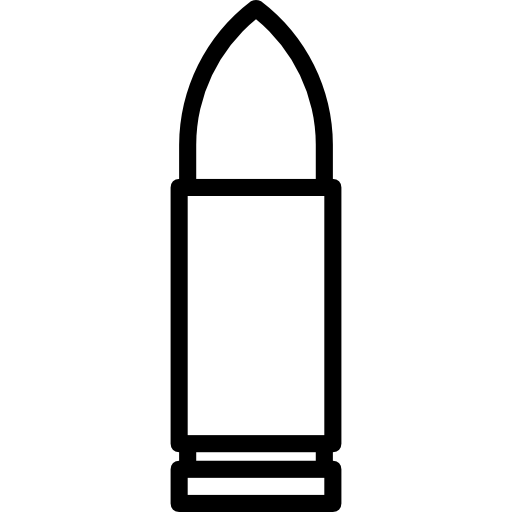
\includegraphics[width=1cm]{chapters/user_manual/resources/bullet.png}       & No effect                                                                             & No effect           \\
        \hline
        
\includegraphics[width=1cm]{chapters/user_manual/resources/pistol.png}       & Fires a bullet if there is one in the inventory. Removes a bullet from the inventory. & No effect           \\
        \hline
        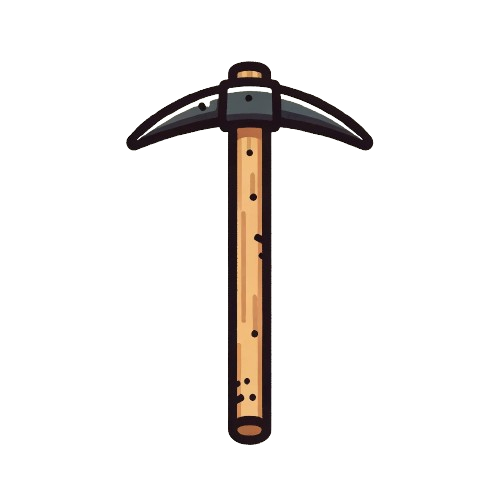
\includegraphics[width=1cm]{chapters/user_manual/resources/pickaxe-slow.png} & Mines slowly.                                                                         & Builds slowly.      \\
        \hline
        
\includegraphics[width=1cm]{chapters/user_manual/resources/pickaxe-mid.png}  & Mines.                                                                                & Builds.             \\
        \hline
        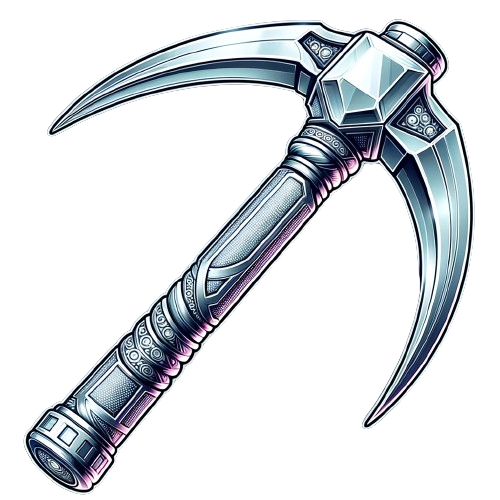
\includegraphics[width=1cm]{chapters/user_manual/resources/pickaxe-fast.png} & Mines quickly.                                                                        & Builds quickly.     \\
        \hline
    \end{tabular}
    \caption{Table of in-game items}
    \label{tab:mytable}
\end{table}

\begin{figure}[h]
    \centering
    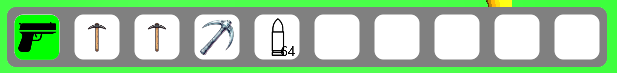
\includegraphics[width=0.8\textwidth]{chapters/user_manual/resources/inventory.png}
    \caption{Inventory}
    \label{fig:inventory}
\end{figure}